% Made up for the tikra benchmark.
\usetikzlibrary{er, positioning}
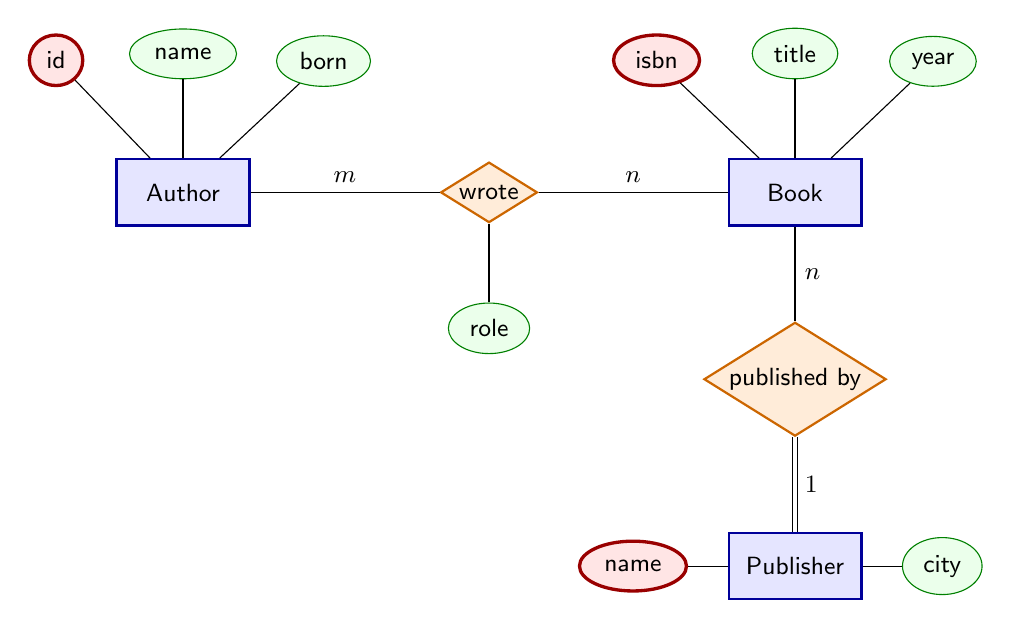
\begin{tikzpicture}[node distance=1cm and 0.5cm, font=\sffamily\small,
    every entity/.style={draw=blue!60!black, fill=blue!10, thick},
    every attribute/.style={draw=green!50!black, fill=green!8},
    key/.style={attribute, draw=red!60!black, fill=red!10, very thick},
    every relationship/.style={draw=orange!80!black, fill=orange!15, thick, aspect=1.6}]
  \node[entity] (author) {Author};
  \node[key, above left=of author] (aid) {id};
  \node[attribute, above=of author] (name) {name};
  \node[attribute, above right=of author] (born) {born};
  \node[relationship, right=2.4cm of author] (wrote) {wrote};
  \node[entity, right=2.4cm of wrote] (book) {Book};
  \node[key, above left=of book] (isbn) {isbn};
  \node[attribute, above=of book] (title) {title};
  \node[attribute, above right=of book] (year) {year};
  \node[relationship, below=1.2cm of book] (pub) {published by};
  \node[entity, below=1.2cm of pub] (publisher) {Publisher};
  \node[key, left=of publisher] (pname) {name};
  \node[attribute, right=of publisher] (city) {city};
  \node[attribute, below=1cm of wrote] (role) {role};
  \foreach \a in {aid, name, born} \draw (author) -- (\a);
  \foreach \a in {isbn, title, year} \draw (book) -- (\a);
  \foreach \a in {pname, city} \draw (publisher) -- (\a);
  \draw (wrote) -- (role);
  \draw (author) -- node[above] {$m$} (wrote);
  \draw (wrote) -- node[above] {$n$} (book);
  \draw (book) -- node[right] {$n$} (pub);
  \draw[double, double distance=1.5pt] (pub) -- node[right] {$1$} (publisher);
\end{tikzpicture}
